\documentclass{article}

 \usepackage[main, preprint]{neurips_2025}

% "preprint" option is used for arXiv or other preprint submissions
 % \usepackage[preprint]{neurips_2025}

\usepackage{amsmath}
\usepackage{graphicx}       % figures
\usepackage[utf8]{inputenc} % allow utf-8 input
\usepackage[T1]{fontenc}    % use 8-bit T1 fonts
\usepackage{url}            % simple URL typesetting
\usepackage{booktabs}       % professional-quality tables
\usepackage{amsfonts}       % blackboard math symbols
\usepackage{nicefrac}       % compact symbols for 1/2, etc.
\usepackage{microtype}      % microtypography
\usepackage{xcolor}         % colors
\usepackage{tabularx}       % tables that fit the text width
\usepackage{float}          % keep tables near their discussion
\usepackage[most]{tcolorbox}
\tcbuselibrary{listings}
\usepackage{hyperref}       % load after float so float anchors are unique

% Load Inconsolata for prompt boxes without changing the document-wide
% monospaced font used by \texttt and \path.
\let\documentttdefault\ttdefault
\usepackage{zi4}
\let\ttdefault\documentttdefault

% Let large figures and tables share pages with the surrounding discussion.
% The defaults are conservative enough to leave conspicuous blank areas when
% several large floats occur close together.
\setcounter{topnumber}{3}
\setcounter{bottomnumber}{2}
\setcounter{totalnumber}{4}
\renewcommand{\topfraction}{0.95}
\renewcommand{\bottomfraction}{0.90}
\renewcommand{\textfraction}{0.05}
\renewcommand{\floatpagefraction}{0.85}

\definecolor{codebackground}{HTML}{EEF1F4}
\definecolor{codeframe}{HTML}{A7AFBA}
\definecolor{codetext}{HTML}{17191C}

\newtcblisting[auto counter]{verbatimblock}[2]{
  enhanced,
  % Keep the complete prompt beside its implementation discussion.
  before={\par\noindent\textbf{Prompt~\thetcbcounter:} #2\par\nobreak\smallskip},
  after=\par\medskip,
  listing only,
  colback=codebackground,
  colframe=codeframe,
  label={#1},
  boxrule=0.5pt,
  arc=1.5mm,
  boxsep=0pt,
  left=5pt,
  right=5pt,
  top=4pt,
  bottom=4pt,
  listing options={
    basicstyle=\fontfamily{zi4}\fontsize{8}{8.2}\selectfont\color{codetext},
    aboveskip=0pt,
    belowskip=0pt,
    breaklines=true,
    breakatwhitespace=true,
    breakindent=0pt,
    breakautoindent=false,
    columns=fullflexible,
    keepspaces=true,
    showstringspaces=false,
    upquote=true,
    literate={-}{{\char45}}1
  }
}

% Note. For the workshop paper template, both \title{} and \workshoptitle{} are required, with the former indicating the paper title shown in the title and the latter indicating the workshop title displayed in the footnote.
\title{GoBench: Evaluating LLMs on the Game of Go}

% The \author macro works with any number of authors. There are two commands
% used to separate the names and addresses of multiple authors: \And and \AND.
%
% Using \And between authors leaves it to LaTeX to determine where to break the
% lines. Using \AND forces a line break at that point. So, if LaTeX puts 3 of 4
% authors names on the first line, and the last on the second line, try using
% \AND instead of \And before the third author name.


\author{%
  Roland Gao\\
  \texttt{gaoroland@gmail.com} \\
}


\begin{document}
\raggedbottom

\maketitle

\begin{abstract}
We introduce GoBench, which evaluates LLMs on full games of $9\times9$ Go and uses KataGo players as Elo anchors.
Without tools, the strongest LLM (GPT-6 Astra) reaches 2500 Elo, while the strongest KataGo player reaches 4400 Elo.
By giving GPT-6 Astra 2 hours of continual learning with coding and evaluation with coding as well, it reaches 3600 Elo.
We aim to keep the GoBench leaderboard up to date as long as it is not saturated: \url{https://rolandgao.com/blog/gobench/}
\end{abstract}

\begin{figure}[H]
  \centering
  % Regenerate from log/summary/results.json: python -m analysis.plot_report_llm_costs --api-only
  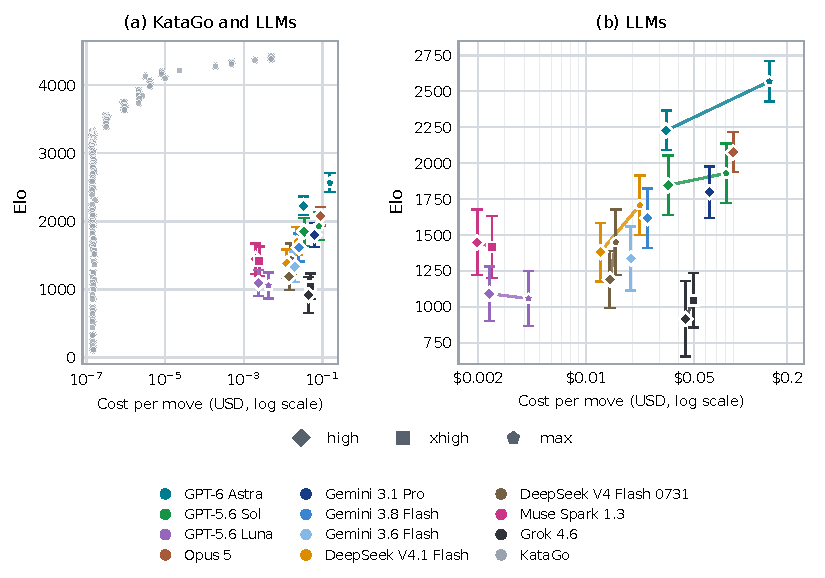
\includegraphics[width=\linewidth]{api_llm_elo_vs_cost.pdf}
  \caption{Elo versus cost per move. \textbf{(a)} 132 KataGo players and LLMs without tools.
  \textbf{(b)} Detail of LLMs. Error bars show 95\% confidence intervals.
  }
  \label{fig:elo-efficiency}
\end{figure}

\clearpage

\section{Introduction}

Current models display ``jagged intelligence'' \citep{karpathy2024jagged} as they approach top human performance in math and coding but lag in other domains.
On our path toward AGI, we want to develop AI systems that can learn new domains at lower cost and with less human supervision.

The game of Go serves as a new domain, and we can evaluate LLMs on Go in a few tracks:
\begin{enumerate}
  \item direct evaluation with no tools
  \item continual learning with coding tools, evaluation with coding tools
  \item continual learning with coding tools, evaluation without tools
  \item continual learning with coding tools and KataGo, evaluation without tools
\end{enumerate}

Humans with no prior Go experience fall into Track 1, while humans with prior Go experience fall into Track 4.
In this work, we focus on Tracks 1 and 2, leaving 3 and 4 to future work, as they require weight updates.

Track 1 measures LLMs' general reasoning ability, as they have not been trained extensively on Go.
As we will show in Section 3.1, Track 1 Elos strongly correlate with ARC-AGI 1/2 scores. GoBench remains far from saturated and can measure general reasoning beyond ARC-AGI \citep{chollet2019measure,chollet2025arcagi2,arcprizefoundation2026leaderboard}.

Track 2 measures LLMs' coding ability and context-based continual learning abilities.
We let the LLMs perform continual learning for $\{0,1,2,4,8\}$ hours before doing the evaluation. This can help us understand the cost of learning a new domain.

We never allow LLMs to call KataGo as a tool during evaluation, as that would defeat the purpose of this evaluation.

\section{Implementation overview}
\label{sec:benchmark-design}

\begin{figure}[hbtp]
  \centering
  % Regenerate: python -m analysis.plot_summary_details
  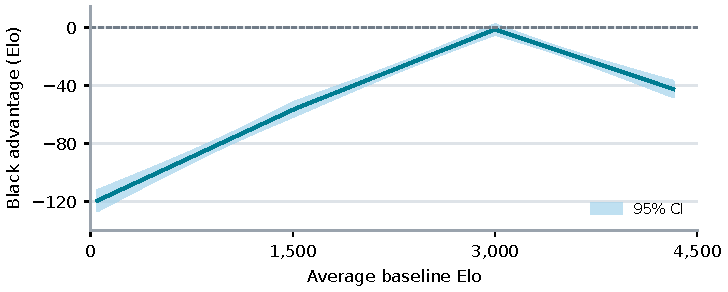
\includegraphics[width=0.88\linewidth]{black_advantage_summary.pdf}
  \caption{Black advantage in the current Elo fit, with its pointwise 95\%
  confidence band. With the 7.0-point komi, Black is at a disadvantage at low Elos, approaches parity at 3000 Elo, and has a slight disadvantage near 4300 Elo.}
  \label{fig:color-functions-plot}
\end{figure}

We provide an implementation overview here with details in the Appendix.

We use the Bradley--Terry model \citep{bradley1952rank} with a Gaussian prior for Elo ratings and confidence intervals.
A relative Elo difference of 400 corresponds to 10:1 odds of winning, and a difference of 800 corresponds to 100:1 odds.
The random player has a fixed Elo of 0, and all other players' Elos are derived from it.

In Go, the Black player goes first and has an advantage.
We mitigate the effect of color by
\begin{enumerate}
  \item having a second game with colors reversed for each selected matchup,
  \item giving the White player 7.0 extra points during scoring,
  \item and predicting the color advantage with a piecewise linear function and incorporating it into the Elo model.
\end{enumerate}

The KataGo players play 320,000 games among themselves to solidify the Elo ladder.
Then, each LLM plays 14 to 30 games to achieve confidence intervals of about $\pm200$.

KataGo's temperature decays exponentially decays from 0.5 to 0.1 to provide some variability in the opening moves.
KataGo players resign after three consecutive evaluations below $-0.95$. The random player never resigns and samples uniformly from the currently legal empty intersections plus pass.

Most KataGo players use \texttt{numPlayouts = 1}, which simply samples from the policy network without any tree search.
For the top four kata1 networks, we also add variants with \texttt{numPlayouts = 60} and
\texttt{numPlayouts = 600}. The strongest KataGo player in our
pool is probably superhuman, but the precise Elos of top human professionals are unknown.

We use $9\times9$ Go boards to get high signal with only a quarter of the cost and time of a $19\times19$ board.
According to the author of KataGo, the $9\times9$ board is far from solved \citep{wu2023katagobooks}; the optimal moves at many positions are still unknown.
We will explore larger board sizes such as $13\times13$ and $19\times19$ once LLMs start saturating the $9\times9$ board.

KataGo timings use a Google Cloud N1 instance (\texttt{n1-custom-1-6656})
with one vCPU, priced at \$0.071 per hour. For the eight players
that use tree search, we estimate time per move by multiplying the measured
single-playout time by the number of playouts.

In the Track 1 API comparison, LLMs use multi-turn reasoning, where reasoning tokens from prior turns are preserved.
This reduces cost while maintaining Elo.
Conversations reset between games or when the context reaches 250K tokens within a game.
Our turn prompt contains complete information, so a conversation reset within a game is acceptable.
We do not use autocompaction because it is not natively supported by all APIs.
If an LLM outputs an illegal move, it is prompted again with the same turn prompt until it succeeds.


\begin{verbatimblock}{prompt:gobench-evaluation}{GoBench evaluation prompt.}
You are playing Black in an ongoing 9x9 Go game against another bot. It is Black to move.

Rules: White komi 7.0, positional superko, passing allowed, self-capture of stones legal. Resolve captures by first removing opposing groups with no liberties, then removing any friendly groups with no liberties. Self-capture remains subject to positional superko. Resigning loses immediately. Two consecutive passes end the game. A draw is worth 0.5 points. Scoring uses strict Tromp-Taylor area scoring with no dead stone removal.

Coordinates: columns A B C D E F G H J from left to right (I is skipped); rows 9 through 1 from top to bottom. B = Black, W = White, Z = empty.

ABCDEFGHJ
9 ZZZZZZZZZ
8 ZZZZZZZZZ
7 ZZZZZZWZZ
6 ZZZZZZZZZ
5 ZZZZBZZZZ
4 ZZZZZZZZZ
3 ZZZZZZZZZ
2 ZZZZZZZZZ
1 ZZZZZZZZZ

Recent 5 moves (oldest to newest): B E5, W G7

Currently illegal because of ko/superko: none

Legal moves: A1, B1, C1, D1, E1, F1, G1, H1, J1, A2, B2, C2, D2, E2, F2, G2, H2, J2, A3, B3, C3, D3, E3, F3, G3, H3, J3, A4, B4, C4, D4, E4, F4, G4, H4, J4, A5, B5, C5, D5, F5, G5, H5, J5, A6, B6, C6, D6, E6, F6, G6, H6, J6, A7, B7, C7, D7, E7, F7, H7, J7, A8, B8, C8, D8, E8, F8, G8, H8, J8, A9, B9, C9, D9, E9, F9, G9, H9, J9, pass, resign

Legal moves is authoritative for the current position and already accounts for ko and positional superko.

Your entire final answer must be one entry copied exactly from Legal moves.
Write that entry on a single line, then end the response immediately.
\end{verbatimblock}

\section{Experimental results}
\label{sec:evaluation}

\subsection{Track 1: LLMs without tools}
We evaluate 18 multi-turn API configurations and one single-turn baseline
without tool calls (Tables~\ref{tab:llm-evaluation-results} and~\ref{tab:context-comparison}). Figure~\ref{fig:elo-efficiency}
shows the multi-turn configurations.
Rank ranges take into account overlapping confidence intervals.


GPT-6 Astra at \texttt{max} leads the Track 1 comparison at $2568\pm140$ Elo and
\$0.154 per move. It is 764 Elo below the fast policy-only KataGo reference
while costing approximately $1.1$ million times more per move. The strongest
KataGo player is 1,859 Elo higher and costs about 31 times less per move.

\begin{table}[htbp]
  \caption{Multi-turn API evaluation results and two KataGo references.
  Illegal moves are counts divided by played moves.}
  \label{tab:llm-evaluation-results}
  \centering
  \footnotesize
  \setlength{\tabcolsep}{3.5pt}
  \renewcommand{\arraystretch}{1.12}
  \begin{tabular}{@{}clrrrlrr@{}}
    \toprule
    Rank & Player (effort) & Elo & 95\% CI & Games &
    \shortstack{Illegal\\moves} &
    \shortstack{Seconds / move} & \shortstack{Cost / move} \\
    \midrule
    1 & GPT-6 Astra (\texttt{max}) & 2568 & $\pm 140$ & 30 & $0/1052$ & 66 & \$0.15 \\
    2--4 & GPT-6 Astra (\texttt{high}) & 2227 & $\pm 138$ & 30 & $0/1015$ & 10 & \$0.033 \\
    2--6 & Opus 5 (\texttt{high}) & 2076 & $\pm 139$ & 30 & $0/1239$ & 26 & \$0.090 \\
    2--8 & GPT-5.6 Sol (\texttt{max}) & 1929 & $\pm 207$ & 14 & $4/516$ & 79 & \$0.081 \\
    3--10 & GPT-5.6 Sol (\texttt{high}) & 1846 & $\pm 207$ & 14 & $24/566$ & 27 & \$0.034 \\
    3--11 & Gemini 3.1 Pro (\texttt{high}) & 1797 & $\pm 178$ & 20 & $1/763$ & 41 & \$0.063 \\
    4--13 & DeepSeek V4.1 Flash (\texttt{max}) & 1707 & $\pm 206$ & 14 & $1/565$ & 140 & \$0.022 \\
    4--13 & Gemini 3.8 Flash (\texttt{high}) & 1616 & $\pm 206$ & 14 & $0/512$ & 13 & \$0.025 \\
    5--17 & DeepSeek V4 Flash 0731 (\texttt{max}) & 1449 & $\pm 227$ & 14 & $160/603$ & 160 & \$0.016 \\
    5--17 & Muse Spark 1.3 (\texttt{high}) & 1449 & $\pm 227$ & 14 & $21/504$ & 46 & \$0.0020 \\
    6--17 & Muse Spark 1.3 (\texttt{xhigh}) & 1415 & $\pm 217$ & 14 & $19/596$ & 38 & \$0.0025 \\
    7--18 & DeepSeek V4.1 Flash (\texttt{high}) & 1380 & $\pm 205$ & 14 & $4/692$ & 70 & \$0.012 \\
    7--18 & Gemini 3.6 Flash (\texttt{high}) & 1336 & $\pm 223$ & 14 & $0/662$ & 5.3 & \$0.020 \\
    9--18 & DeepSeek V4 Flash 0731 (\texttt{high}) & 1189 & $\pm 197$ & 14 & $3/544$ & 150 & \$0.014 \\
    9--18 & GPT-5.6 Luna (\texttt{high}) & 1091 & $\pm 190$ & 14 & $3/806$ & 17 & \$0.0024 \\
    9--18 & GPT-5.6 Luna (\texttt{max}) & 1058 & $\pm 189$ & 14 & $0/800$ & 32 & \$0.0043 \\
    9--18 & Grok 4.6 (\texttt{xhigh}) & 1044 & $\pm 189$ & 14 & $9/500$ & 35 & \$0.050 \\
    12--18 & Grok 4.6 (\texttt{high}) & 916 & $\pm 263$ & 14 & $19/551$ & 30 & \$0.044 \\
    \midrule
    -- & KataGo (fast policy) & 3332 & $\pm 32$ & 4002 & -- & 0.0072 & \(\$1.4\times10^{-7}\) \\
    -- & KataGo (highest Elo) & 4427 & $\pm 35$ & 2992 & -- & 250 & \$0.0049 \\
    \bottomrule
  \end{tabular}
\end{table}

\paragraph{Single-turn versus multi-turn context.}
For GPT-6 Astra at \texttt{high}, multi-turn context reduces time by a factor of four and cost by 40\% while maintaining Elo.

\begin{table}[htbp]
  \caption{GPT-6 Astra at \texttt{high}: single-turn versus multi-turn context.
  Both configurations have zero reported illegal moves and API problems.
  Cached input is the fraction of input tokens served from cache.}
  \label{tab:context-comparison}
  \centering
  \small
  \setlength{\tabcolsep}{5pt}
  \renewcommand{\arraystretch}{1.12}
  \begin{tabular}{@{}lrrrrrr@{}}
    \toprule
    Context & Elo (95\% CI) & Games & \shortstack{Cached\\input} &
    \shortstack{Output tokens\\per move} & \shortstack{Seconds / move} &
    \shortstack{Cost / move} \\
    \midrule
    Single-turn & $2011\pm217$ & 14 & 0.00\% & 1070.49 & 44.70 & \$0.0581 \\
    Multi-turn & $2227\pm138$ & 30 & 89.50\% & 196.61 & 10.32 & \$0.0332 \\
    \bottomrule
  \end{tabular}
\end{table}

\paragraph{Correlation with ARC-AGI.}

As shown in Figure~\ref{fig:arc-agi}, LLMs' Track 1 Elos strongly correlate with their ARC-AGI scores.

\begin{figure}[htbp]
  \centering
  % Data: data/arc_agi/evaluations.json
  % Regenerate: python -m analysis.plot_arc_agi_correlation
  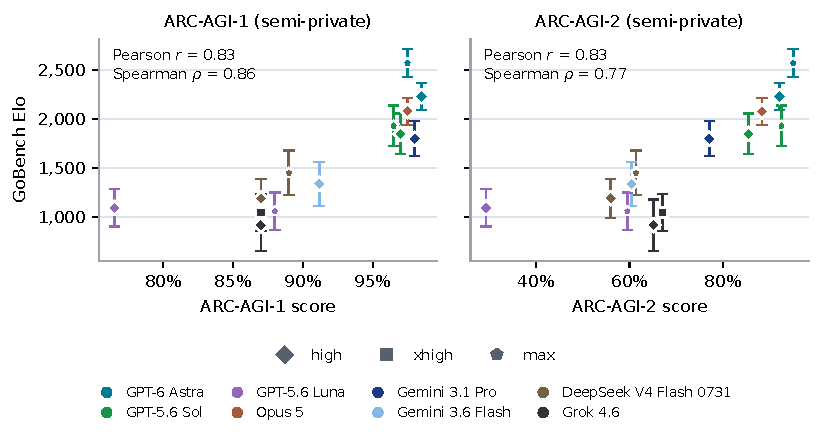
\includegraphics[width=\linewidth]{arc_agi_correlation.pdf}
  \caption{GoBench Elo versus ARC-AGI-1 and ARC-AGI-2 semi-private scores.}
  \label{fig:arc-agi}
\end{figure}

\subsection{Track 2: LLMs with coding tools}

In Track 2, the model performs continual learning for $N\in\{0,1,2,4,8\}$ hours and is then evaluated with the resulting context checkpoint.
Each evaluation game starts from the same context checkpoint, which does not include changes made during prior evaluation games.
The model may further update the context during the evaluation game. Each evaluation game is capped at 30 minutes, and exceeding the cap counts as a loss.
The remaining time is always available to the agent through a continuously updated \texttt{clock.json} file and in the turn prompt.

Continual learning can mean updating weights or context. In this work, we update the LLM's context while keeping its weights fixed.
Context can be thought of as files and directories in a file system, and it is synonymous with agentic harness state.

We evaluate Codex with GPT-6 Astra and GPT-5.6 Sol, both at \texttt{high}. We disable internet access
and access to KataGo source code and results, while allowing other local tools.
We use Bubblewrap as the sandbox and limit the compute resources to one physical CPU core, 4GB of RAM, and 2GB of disk.
The Codex process is inside the sandbox, and it reaches the OpenAI API endpoint through a reverse proxy over a Unix domain socket.
The socket messages are logged so that further investigation can be conducted to check for cheating, such as trying to reach the internet.

We considered giving the model access to KataGo during the continual learning phase,
but we eventually decided against this idea because the model would just create an opening book by using the best KataGo model. 

As shown in Figure~\ref{fig:learning-time},
GPT-6 Astra in Codex with 0 hours of continual learning matches the best-performing model from Track 1.
Its Elo improves with 1h and 2h of continual learning, while the 4h and 8h runs show no improvement beyond the 2h run.

GPT-5.6 Sol improves as continual learning duration increases from 0h to 1h, but it degrades as duration increases to 2h, 4h, 8h.

By using coding tools, they built C++ Go engines with Monte Carlo tree search, tactical rules, learned move-selection policies, and precomputed opening books, then used them to choose moves during evaluation.

The reverse proxy logs showed no signs of internet access attempts.

\begin{figure}[htbp]
  \centering
  % Regenerate: python -m analysis.plot_summary_details
  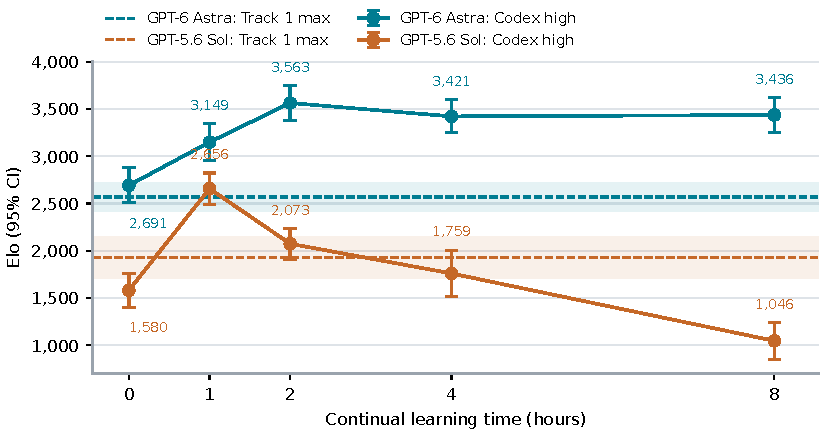
\includegraphics[width=\linewidth]{codex_learning_time.pdf}
  \caption{GPT-6 Astra and GPT-5.6 Sol at \texttt{high} in Codex after 0--8 hours of continual learning.
  Error bars show 95\% confidence intervals. Dashed lines and shaded
  bands show each model's Track 1 \texttt{max} baseline.}
  \label{fig:learning-time}
\end{figure}

\subsection{Manually inspecting the LLM games}
Manually inspecting the LLM games revealed two potential concerns, positional
superko and KataGo's passing behavior, and we wrote a checker for each.

The Go Text Protocol (GTP) is the interface used for games between KataGo and LLMs, but the engine's
GTP \texttt{play} command accepted moves that violate positional superko. We implemented our own checker to prevent
illegal moves and reran the experiments after identifying violations in an
earlier set of games.

Strict area scoring has no automatic dead stone removals,
but KataGo players around 2000 Elos are very likely to pass while leaving opponent's dead stones unremoved.
This behaviour disappears as the KataGo players achieve over 3000 Elo, as shown in Figure~\ref{fig:passing-errors}.

\begin{figure}[htbp]
  \centering
  % Data: data/audits/passing/passing_b6c96_temp01.json
  % Regenerate: python -m analysis.plot_passing_errors
  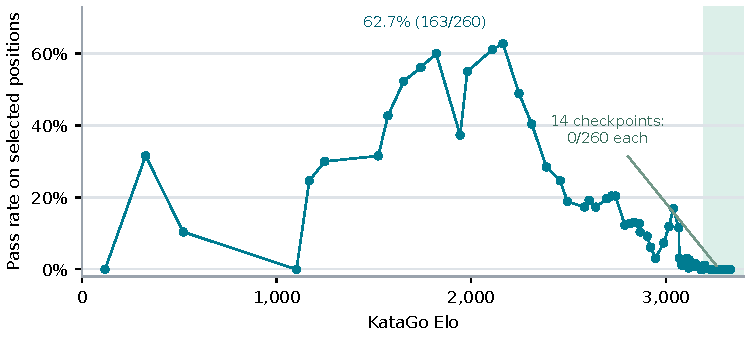
\includegraphics[width=0.9\linewidth]{katago_passing_errors.pdf}
  \caption{Pass rates on 13 historical positions across 63 KataGo
  \texttt{b6c96} checkpoints.}
  \label{fig:passing-errors}
\end{figure}



\section{Related work}

Go has long served as a testbed for artificial intelligence. AlphaGo combined
deep neural networks with tree search to achieve superhuman performance
\citep{silver2016alphago}, while AlphaZero learned Go, chess, and shogi through
self-play without expert demonstrations \citep{silver2018alphazero}. KataGo
subsequently improved the efficiency of self-play training and is open source \citep{wu2019katago}.

KataGo-Bench-1K \citep{ma2026logos} contains 1,000 board states and scores next-move predictions using KataGo as the judge. However, it does not involve complete games, providing only a myopic view of the players' strengths.

Several active benchmarks evaluate LLMs through games and puzzles. Kaggle Game Arena, the AI Chess Leaderboard, and LLM CHESS evaluate performance on chess \citep{kaggle2026gamearena,dubesor2026leaderboard,kolasani2025llmchess}; GTO Wizard Benchmark evaluates performance on poker \citep{provost2026gtowizard}; and ARC-AGI-3 and MazeBench evaluate performance on puzzle games \citep{arcprizefoundation2026arcagi3,rodriguezsalgado2026pixels}.
To our knowledge, GoBench is the first benchmark evaluating LLMs' performance on complete games of Go, providing a novel addition to the set of benchmarks.

\section{Directions for future work}

\paragraph{Continual learning with weight updates.}
We experimented only with continual learning through context updates.
Weight updates are necessary for Tracks 3 and 4, where the LLM performs continual learning with tools but is evaluated without tools.
Track 4 matches the environment in which human professionals play Go, and it is essential for measuring LLMs' learning efficiency relative to that of humans.

\paragraph{Adversarial robustness.}
Superhuman KataGo networks have been defeated by substantially weaker agents using adversarial strategies
\citep{wang2023adversarial}.
We can similarly study whether LLMs are susceptible to adversarial attacks in the game of Go,
and whether they can be trained to achieve adversarial robustness.

\paragraph{Video game benchmarks.}
GoBench evaluates reasoning on text.
Future benchmarks can further incorporate visual perception
and physical control, providing a path toward physical intelligence.

% \paragraph{Continual Learning}
% Since learning can happen by updating either the weights or the context,
% an agentic harness that updates the context could be sufficient for saturating GoBench given enough compute for learning.
% For example, the agentic harness can spend large amounts of compute on tree searches and distill the conclusions into a table.
% During a game, most moves can be decided by simply performing a table lookup, and novel game states can be computed on the fly with the result written to the table again.
% Since the table might become huge, baking the table back into the weights can achieve compression, and table entries where the updated weights can handle can be removed.

% Start the bibliography on its own page.
\clearpage
\bibliographystyle{plainnat}
\bibliography{references}

\clearpage
\appendix
\small

\section{Color function}
We introduce a color function that estimates the Black advantage given the average Elo of the two players.
We first fit a Bradley--Terry Elo model without a color function and denote its
ratings by $b_i$. In the second stage, we fit the final player ratings and the color function while keeping $b_i$ frozen.

We conduct an ablation study to find the best color function.
To understand its generalization to unseen player matchups, we conduct the train-test split not by game, but by player.
We randomly select half of the players, assign the matchups between them as the train set, and assign the rest of the games as the test set.
Given 133 KataGo players and 300K games, we estimate $b_i$ for all the players first,
and then calculate mean train and test losses over 40 repetitions of train-test sampling.
This ablation uses an earlier 300K-game dataset. The current historical rating pool is listed in
Appendix~\ref{app:katago-players}; both pools include the random anchor and
\texttt{kata1-zhizi-b40c768nbt-fdx6c}.


The results are shown in Table~\ref{tab:color-function-ablation}.
We mark a color function as statistically worse than the quadratic one when
the 95\% Student's $t$ interval over its 40 paired test-loss differences lies
entirely above zero. A one-Elo knot spacing that overfits the train set generalizes poorly to the test set, as expected.
We use the piecewise-linear color function for its simplicity; its test loss ties with the quadratic.

\begin{table}[htbp]
  \caption{Ablation study on the color function.}
  \label{tab:color-function-ablation}
  \centering
  \small
  \renewcommand{\arraystretch}{1.08}
  \setlength{\tabcolsep}{4pt}
  \begin{tabular}{@{}lrrrc@{}}
    \toprule
    Color function & Color params & Train loss & Test loss & Worse than quadratic? \\
    \midrule
    Piecewise linear (1,500 Elo)     &    4 & 0.3658 & $\mathbf{0.3664}$ & No \\
    Quadratic                        &    3 & 0.3660 & $\mathbf{0.3664}$ & No \\
    Piecewise constant (500 Elo)     &    9 & 0.3657 & 0.3667 & No \\
    Negative exponential             &    2 & 0.3662 & 0.3668 & Yes \\
    Cubic spline                     &    8 & 0.3653 & 0.3674 & Yes \\
    Piecewise linear (500 Elo)       &   10 & 0.3653 & 0.3676 & Yes \\
    Piecewise constant (250 Elo)     &   17 & 0.3652 & 0.3676 & Yes \\
    Piecewise linear (250 Elo)       &   18 & 0.3649 & 0.3676 & Yes \\
    Global color term                &    1 & 0.3683 & 0.3677 & Yes \\
    No color term                    &    0 & 0.3709 & 0.3699 & Yes \\
    Piecewise linear (1 Elo)         & 4,270 & $\mathbf{0.3521}$ & 0.4894 & Yes \\
    \bottomrule
  \end{tabular}
\end{table}


Even though using the color function has negligible influence on the ranking of the players, it improves the predicted win probabilities, as shown by the better test loss in Table~\ref{tab:color-function-ablation}.


\section{Elo estimation and uncertainty}
\label{app:elo-estimation}

This appendix gives the statistical details of the two-stage Elo model described
in Section~\ref{sec:benchmark-design}. In the first stage, we fit a Bradley--Terry model without a color
term to obtain baseline ratings $b_i$. These ratings are then frozen. In the
second stage, we jointly fit the reported ratings $r_i$ and the parameters of
the Black-advantage function $f$.

\subsection{Outcome model}

If $r_i$ is the Elo rating of player $i$, then the probability that player $i$ wins as Black against player $j$ is

\[
p_{ij}
=
\sigma\!\left(
c\left[
r_i-r_j+f((b_i+b_j)/2)
\right]
\right),
\qquad
c=\frac{\ln 10}{400},\quad \sigma(x)=\frac{1}{1+\exp(-x)},
\]
where $b_i$ and $b_j$ are the frozen first-stage baseline ratings and
$f$ is the color function.

\subsection{Maximum a posteriori estimation}

Given a list of game results $G = [(i,j,y),\ldots]$, where player $i$ is Black, player $j$ is White, and $y$ is the game result in $\{1,0,1/2\}$, we estimate the Elo ratings by maximizing the regularized Bradley--Terry log-likelihood

\[
\mathcal{L}(\boldsymbol{\theta})
=
\sum_{(i,j,y)\in G}
\left[
y\log p_{ij}+(1-y)\log(1-p_{ij})
\right]
-\frac{1}{2}
\sum_k\frac{(\theta_k-\mu_k)^2}{s_k^2},
\]
where $\boldsymbol{\theta}$ includes both player ratings and Black-advantage
parameters, and $\mu_k$ and $s_k$ are the mean and standard deviation of the
independent Gaussian prior on parameter $k$.

For the Gaussian prior, we use $N(0, 10000^2)$ for both KataGo player ratings and color-function parameters, but $N(1000, 2000^2)$ for LLMs to speed up their convergence.


\subsection{Laplace confidence intervals}

Uncertainty in the fitted parameters is approximated using a Laplace
approximation \citep{tierney1986accurate} around the maximum a posteriori estimate
\(\widehat{\boldsymbol{\theta}}\). The information matrix at the fitted
parameters is
\[
\widehat{\boldsymbol{I}}
=
c^2\sum_g
\widehat{p}_g(1-\widehat{p}_g)
\boldsymbol{x}_g\boldsymbol{x}_g^\mathsf{T},
\]
where \(\boldsymbol{x}_g\) denotes the fixed second-stage feature vector for
game \(g\). Its player components are \(+1\) for the Black player and \(-1\)
for the White player, and its color components are the piecewise-linear basis
values evaluated at the frozen average baseline Elo.


Including the curvature of the independent Gaussian priors, the negative
Hessian of the log posterior is
\[
\widehat{\boldsymbol{H}}
=
\widehat{\boldsymbol{I}}
+
\operatorname{diag}(s_1^{-2},\ldots,s_d^{-2}),
\]
where \(d\) is the number of optimized parameters. The approximate posterior
covariance matrix is \(\boldsymbol{C}=\widehat{\boldsymbol{H}}^{-1}\), and the
marginal \(95\%\) confidence interval is
\[
\widehat{r}_i
\pm
1.96\sqrt{C_{ii}}.
\]

These intervals are conditional on the frozen baseline ratings; they do not
propagate uncertainty from the first-stage no-color fit.

The player with the random policy is fixed at 0 Elo as an anchor and is not
optimized in $\boldsymbol{\theta}$ or included in the covariance matrix.

\subsection{Limitations of the Elo model}
Elo ratings hide non-transitive effects, where a low-Elo player beats a high-Elo player with more than $50\%$ probability.
Displaying game outcomes between all players in a 2D matrix can be beneficial, but we stick to Elo for its simplicity.


\section{Matchmaking}
We want to schedule games that shrink the confidence intervals as much as possible.
To do this, we first introduce the gain matrix, where each entry $(i,j)$ is defined as the predicted reduction in the sum of confidence intervals of players we care about:

\[
G_{ij}
=
\sum_{q\in\mathcal{S}}
\left[
\sqrt{C_{qq}}
-
\sqrt{C^{(ij)}_{qq}}
\right],
\]

where $C^{(ij)}$ is the predicted covariance matrix after players $i$ and $j$ play a pair of color-swapped games, and $\mathcal{S}$ is the set of players we care about.


The games are scheduled in batches, and the games within a batch are played concurrently.
Before each batch, the Elo ratings, confidence intervals, and gain matrices are recalculated using all completed games.

In the first stage, the KataGo players play a total of 320K games among themselves in batches of 4K.
In each batch, 2K color-swapped pairs are sampled with probability proportional to the gain of each pair.

In the second stage, LLMs play against KataGo in batches of two color-swapped
games. In total, LLMs play 420 games: 320 API games across 19
configurations (14--30 games each) and 100 Codex games across five continual-learning
budgets (20 each). In each batch, the pair that maximizes the gain is chosen.

Why are the matchmaking algorithms different for the two stages?
The ground-truth gain matrix is calculated only before every batch.
Predicting the gain matrix after $N$ games requires modeling up to $3^N$ possible outcomes, given 3 potential outcomes per game.
Because predicting the gain matrix is intractable, we simply sample with probability proportional to the gain.
As an added benefit, such sampling is more robust to the non-transitivity in the Elo model.

The final 95\% confidence-interval half-widths are 16--36 Elo for non-anchor KataGo players and 138--263 Elo for LLMs.

\clearpage
\section{KataGo player pool}
\label{app:katago-players}

Table~\ref{tab:katago-players} lists every KataGo player used as an Elo anchor.
Names of the form \texttt{bAcB-sN} identify a KataGo network with $A$ residual
blocks and $B$ channels after $N$ training steps. An \texttt{x2} suffix marks a
network trained with two GPUs for gradients instead of one, and \texttt{nbt} marks the
newer nested-bottleneck architecture. A \texttt{-p$P$} suffix denotes tree
search with $P$ playouts; players without one use \texttt{numPlayouts = 1}.

A \texttt{-temp-$T$} suffix changes the policy-sampling temperature schedule of
Section~\ref{sec:benchmark-design}, which by default decays from $0.5$ to $0.1$.
For $T \neq 0.3$, the suffix pins the temperature to the constant $T$ for the whole
game. The single exception is $T = 0.3$, which keeps the decaying schedule but
raises its floor, decaying from $0.5$ to $0.3$. The purpose is to make the low-Elo population denser.

\begin{table}[htbp]
  \caption{The 133 KataGo players in the historical rating pool, ordered by Elo. Player
  names omit the \texttt{kata1-} prefix and the \texttt{-d\textit{N}} data-count
  segment; \texttt{random} is the uniform-random anchor fixed at 0 Elo. CI is the
  half-width of the 95\% confidence interval. The Zhizi network lacks a timing
  measurement and is omitted only from the cost plot.}
  \label{tab:katago-players}
  \centering
  \scriptsize
  \setlength{\tabcolsep}{2.5pt}
  \begin{tabular}{@{}lrr@{\hspace{14pt}}lrr@{\hspace{14pt}}lrr@{}}
    \toprule
    Player & Elo & CI & Player & Elo & CI & Player & Elo & CI \\
    \midrule
    \texttt{b28c512nbt-s8566598912-p600} & 4427 & 35 & \texttt{b6c96-s141089536} & 3302 & 32 & \texttt{b6c96-s16525312-temp-0.5} & 2160 & 27 \\
    \texttt{b28c512nbt-s12313658112-p600} & 4385 & 35 & \texttt{b6c96-s130521856} & 3297 & 31 & \texttt{b6c96-s14649344} & 2110 & 29 \\
    \texttt{b28c512nbt-s7229617920-p600} & 4384 & 35 & \texttt{b6c96-s115648256} & 3290 & 31 & \texttt{b6c96-s14649344-temp-0.3} & 2084 & 27 \\
    \texttt{b18c384nbt-s9761732864-p600} & 4368 & 35 & \texttt{b6c96-s103950080} & 3275 & 31 & \texttt{b6c96-s16525312-temp-0.7} & 2011 & 27 \\
    \texttt{b28c512nbt-s12313658112-p60} & 4346 & 34 & \texttt{b6c96-s108812288} & 3270 & 31 & \texttt{b6c96-s13733120-temp-0.3} & 1985 & 27 \\
    \texttt{b28c512nbt-s8566598912-p60} & 4332 & 34 & \texttt{b6c96-s95425792} & 3260 & 31 & \texttt{b6c96-s13733120} & 1980 & 29 \\
    \texttt{b28c512nbt-s7229617920-p60} & 4308 & 34 & \texttt{b6c96-s89508352} & 3249 & 31 & \texttt{b6c96-s12849664} & 1943 & 28 \\
    \texttt{b18c384nbt-s9761732864-p60} & 4278 & 34 & \texttt{b6c96-s83588096} & 3248 & 31 & \texttt{b6c96-s13733120-temp-0.5} & 1924 & 26 \\
    \texttt{zhizi-b40c768nbt-fdx6c} & 4216 & 36 & \texttt{b6c96-s73091584} & 3228 & 31 & \texttt{b6c96-s12849664-temp-0.5} & 1856 & 26 \\
    \texttt{b28c512nbt-s12313658112} & 4199 & 34 & \texttt{b6c96-s78659584} & 3227 & 31 & \texttt{b6c96-s11888896} & 1820 & 26 \\
    \texttt{b28c512nbt-s8566598912} & 4191 & 34 & \texttt{b6c96-s69427456} & 3198 & 31 & \texttt{b6c96-s11888896-temp-0.5} & 1742 & 26 \\
    \texttt{b28c512nbt-s7229617920} & 4161 & 34 & \texttt{b6c96-s65341184} & 3189 & 31 & \texttt{b6c96-s10825472} & 1742 & 28 \\
    \texttt{b18c384nbt-s9761732864} & 4131 & 34 & \texttt{b6c96-s59560704} & 3180 & 31 & \texttt{b6c96-s14649344-temp-0.9} & 1676 & 26 \\
    \texttt{b60c320-s6678602752} & 4102 & 34 & \texttt{b6c96-s63439616} & 3168 & 31 & \texttt{b6c96-s10014464} & 1654 & 27 \\
    \texttt{b40c256-s11840935168} & 4071 & 34 & \texttt{b6c96-s55682304} & 3152 & 31 & \texttt{b6c96-s10014464-temp-0.3} & 1619 & 25 \\
    \texttt{b40c256-s8049900800} & 4063 & 34 & \texttt{b6c96-s56669696} & 3147 & 31 & \texttt{b6c96-s13733120-temp-0.9} & 1583 & 25 \\
    \texttt{b40c256x2-s4120339456} & 4027 & 34 & \texttt{b6c96-s52864512} & 3119 & 31 & \texttt{b6c96-s8982784} & 1572 & 27 \\
    \texttt{b40c256-s5793846528} & 3994 & 34 & \texttt{b6c96-s50894592} & 3117 & 31 & \texttt{b6c96-s8080640} & 1523 & 27 \\
    \texttt{b40c256x2-s4833666560} & 3987 & 33 & \texttt{b6c96-s48921344} & 3110 & 31 & \texttt{b6c96-s8982784-temp-0.3} & 1519 & 25 \\
    \texttt{b20c256x2-s5055114240} & 3931 & 34 & \texttt{b6c96-s46949632} & 3082 & 31 & \texttt{b6c96-s8080640-temp-0.3} & 1413 & 24 \\
    \texttt{b20c256x2-s3354994176} & 3898 & 33 & \texttt{b6c96-s45189632} & 3070 & 30 & \texttt{b6c96-s8982784-temp-0.5} & 1364 & 24 \\
    \texttt{b20c256x2-s2430231552} & 3861 & 33 & \texttt{b6c96-s43286272} & 3066 & 31 & \texttt{b6c96-s6127360} & 1248 & 26 \\
    \texttt{b20c256x2-s1610809600} & 3847 & 33 & \texttt{b6c96-s41312768} & 3038 & 31 & \texttt{b6c96-s8080640-temp-0.5} & 1246 & 23 \\
    \texttt{b20c256x2-s1039565568} & 3841 & 33 & \texttt{b6c96-s39339776} & 3016 & 30 & \texttt{b6c96-s5214720} & 1168 & 26 \\
    \texttt{b20c256x2-s668214784} & 3797 & 33 & \texttt{b6c96-s37368064} & 2989 & 31 & \texttt{b6c96-s8982784-temp-0.7} & 1137 & 23 \\
    \texttt{b15c192-s1062526208} & 3752 & 33 & \texttt{b6c96-s35356160} & 2947 & 30 & \texttt{b6c96-s4136960} & 1103 & 22 \\
    \texttt{b15c192-s798345984} & 3750 & 33 & \texttt{b6c96-s33239552} & 2921 & 31 & \texttt{b6c96-s10014464-temp-0.9} & 1062 & 22 \\
    \texttt{b20c256-s241116160} & 3736 & 33 & \texttt{b6c96-s32344832} & 2904 & 30 & \texttt{b6c96-s8080640-temp-0.7} & 996 & 22 \\
    \texttt{b15c192-s449394432} & 3700 & 33 & \texttt{b6c96-s30394624} & 2867 & 31 & \texttt{b6c96-s4136960-temp-0.3} & 917 & 22 \\
    \texttt{b15c192-s315428352} & 3689 & 33 & \texttt{b6c96-s31390976} & 2864 & 31 & \texttt{b6c96-s5214720-temp-0.5} & 859 & 21 \\
    \texttt{b15c192-s230670592} & 3638 & 33 & \texttt{b6c96-s29422336} & 2838 & 30 & \texttt{b6c96-s4136960-temp-0.5} & 731 & 20 \\
    \texttt{b15c192-s172540416} & 3636 & 33 & \texttt{b6c96-s28460288} & 2815 & 31 & \texttt{b6c96-s5214720-temp-0.7} & 693 & 20 \\
    \texttt{b10c128-s501483520} & 3565 & 32 & \texttt{b6c96-s27415296} & 2789 & 30 & \texttt{b6c96-s6127360-temp-0.9} & 640 & 19 \\
    \texttt{b10c128-s356821760} & 3556 & 32 & \texttt{b6c96-s26363136} & 2741 & 31 & \texttt{b6c96-s4136960-temp-0.7} & 563 & 19 \\
    \texttt{b10c128-s182492416} & 3535 & 32 & \texttt{b6c96-s25461504} & 2721 & 30 & \texttt{b6c96-s1995008} & 521 & 22 \\
    \texttt{b10c128-s258941696} & 3529 & 32 & \texttt{b6c96-s24455424} & 2696 & 31 & \texttt{b6c96-s4136960-temp-0.9} & 440 & 17 \\
    \texttt{b10c128-s146897408} & 3508 & 32 & \texttt{b6c96-s23401472} & 2640 & 29 & \texttt{b6c96-s1995008-temp-0.3} & 328 & 16 \\
    \texttt{b10c128-s108710656} & 3494 & 32 & \texttt{b6c96-s22371328} & 2606 & 31 & \texttt{b6c96-s938496} & 327 & 21 \\
    \texttt{b10c128-s82632704} & 3459 & 32 & \texttt{b6c96-s21371392} & 2582 & 29 & \texttt{b6c96-s938496-temp-0.3} & 235 & 16 \\
    \texttt{b10c128-s56992512} & 3438 & 32 & \texttt{b6c96-s20302336} & 2494 & 31 & \texttt{b6c96-s1995008-temp-0.9} & 168 & 16 \\
    \texttt{b10c128-s41138688} & 3388 & 32 & \texttt{b6c96-s19408128} & 2458 & 29 & \texttt{b6c96-s1248000} & 119 & 20 \\
    \texttt{b6c96-s175395328} & 3332 & 32 & \texttt{b6c96-s18429184} & 2386 & 29 & \texttt{b6c96-s1248000-temp-0.3} & 113 & 16 \\
    \texttt{b6c96-s152505856} & 3314 & 32 & \texttt{b6c96-s17434112} & 2311 & 28 & \texttt{random} & 0 & 0 \\
    \texttt{b6c96-s165180416} & 3312 & 31 & \texttt{b6c96-s16525312} & 2246 & 28 &  &  &  \\
    \texttt{b6c96-s122554112} & 3304 & 32 & \texttt{b6c96-s15704832} & 2164 & 29 &  &  &  \\
    \bottomrule
  \end{tabular}
\end{table}

\end{document}
